%%%%%%%%%%%%%%%%%%%%% Chapter 19 %%%%%%%%%%%%%%%%%%%%%%%%%%%%%%%%%
% Machine Unlearning: The Right to be Forgotten
%%%%%%%%%%%%%%%%%%%%%%%%%%%%%%%%%%%%%%%%%%%%%%%%%%%%%%%%%%%%%%%%%
\motto{Machine Unlearning is the process of removing data influence from a trained model without starting from scratch. It is the technical fulfillment of the Right to be Forgotten.}

\chapter{Machine Unlearning: The Right to be Forgotten}
\label{chap:machine_unlearning}

\abstract{As global regulations like the GDPR and Vietnam's Decree 13/2023 grant users the "Right to be Forgotten," the Trustworthy AI Architect must go beyond simple database deletions. This chapter introduces the emerging field of Machine Unlearning---technical methods for removing the influence of specific training records from already-deployed models. We analyze the differences between exact retraining and approximate unlearning using influence functions and the Hessian matrix. We also explore the unique challenges of unlearning in distributed systems and Large Language Models, where "forgetting" a sample must be balanced against maintaining overall model stability.}

\section{When Users Ask to be Forgotten}
\label{sec:unlearning_intro_ch17}

In a world governed by privacy regulations, removing a user's raw data from a database is often legally insufficient if that data's "signature" remains embedded within a trained machine learning model. If a model can still produce an output that depends specifically on a deleted record, the user has not truly been forgotten.

\textbf{Machine Unlearning} is the process of updating a model such that its weights reflect what they would have been if the "forgotten" data point had never existed, without the prohibitive cost of retraining the entire model from scratch.

\section{Core Unlearning Methodologies}
\label{sec:unlearning_methods_ch17}

The choice of unlearning method depends on the required strength of the guarantee and the computational budget:

\begin{description}
  \item[Exact Unlearning (Retraining):] 
        The perfectly compliant approach. The model is retrained on the dataset $D \setminus D_f$. While providing a perfect guarantee, it is $O(N)$ and becomes computationally prohibitive for Large Language Models or massive industrial datasets.
  \item[Approximate Unlearning (Influence Functions):]
        For many deep learning models, we can estimate the \textit{influence} of a specific data point $D_f$ on the model parameters $\theta$ and update the weights inversely. This is often calculated using the inverse of the Hessian matrix:
        \begin{equation}
        \theta_{\text{new}} = \theta_{\text{old}} + \epsilon \cdot H^{-1} \sum_{x \in D_f} \nabla_\theta L(\theta_{\text{old}}, x)
        \end{equation}
\end{description}

\begin{figure}[t]
\centering
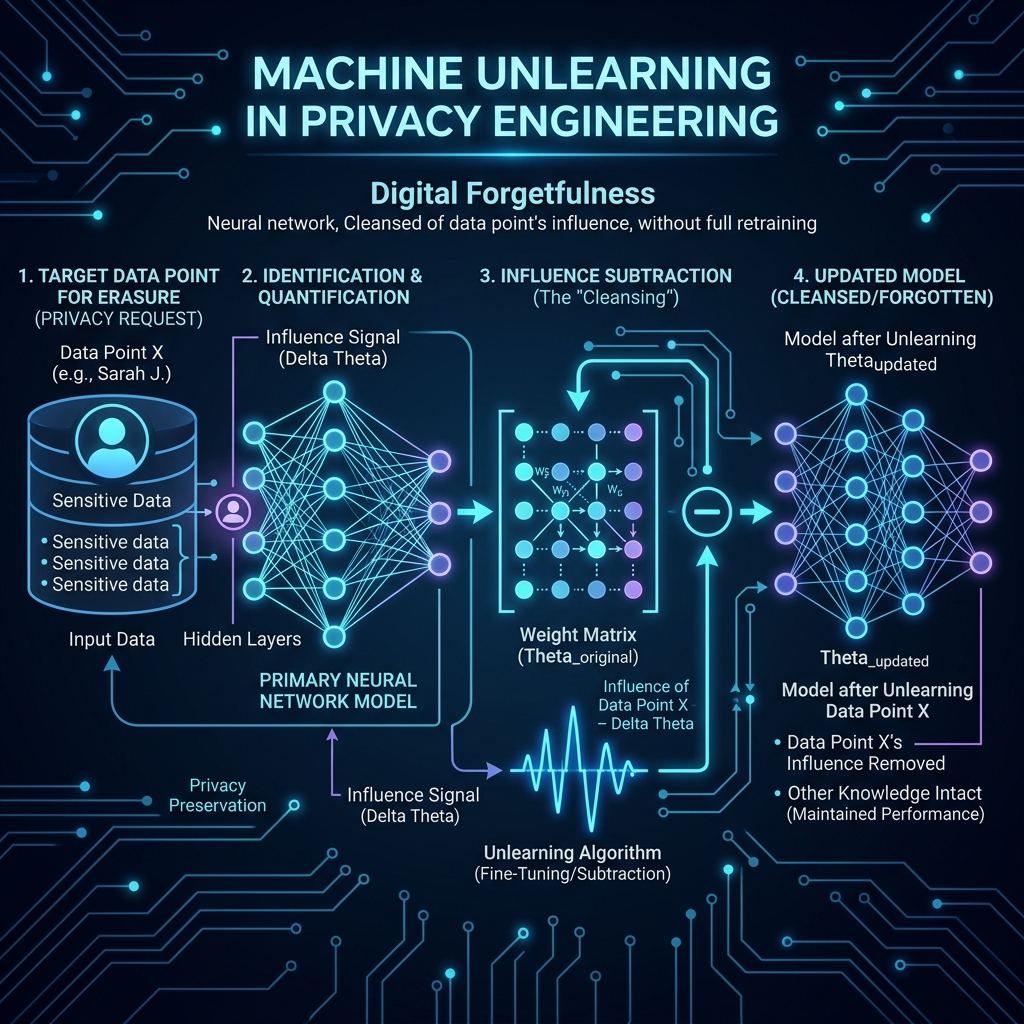
\includegraphics[width=0.9\textwidth]{figures/ch17_unlearning.png}
\caption{Machine Unlearning in Privacy Engineering: The process of digitally erasing a data point's influence from model weights to satisfy the 'Right to be Forgotten'.}
\label{fig:ch17_unlearning}
\end{figure}

\section{Unlearning in Distributed Systems}
\label{sec:federated_unlearning_ch17}

In Federated Learning environments, unlearning becomes even more complex. The server must remove a specific client's contribution without ever having had access to their raw data. This is typically achieved through \textbf{Federated Unlearning} protocols, where the aggregator subtracts a normalized version of the client's historical updates and performs a small number of "repair" rounds to re-stabilize the global model.

\section{Implementation: Gradient Ascent}
\label{sec:gradient_ascent_ch17}

A simple, albeit potentially unstable, implementation of unlearning involves "undoing" the training step through gradient ascent on the forget set. By maximizing the loss on the data points we wish to forget, we move the model weights away from those specific patterns. However, to prevent the model from collapsing, this must be combined with regularization that keeps the weights close to their original values for the remainder of the dataset.

\section{Conclusion}
\label{sec:conclusion_unlearning_ch17}

Part V has explored the modern frontier of Artificial Intelligence. We have seen how LLMs require new privacy defenses (Chapter 15), how multimodal fusion introduces hidden risks (Chapter 16), and how we can implement the technical "Right to be Forgotten" (Chapter 17). 

As we move into the final part of this book, Part VI, we shift our perspective from the internal defenses of the model to the \textbf{Verifiable Architecture} of the entire system, exploring how to prove trust through cryptography and formal logic.


